\documentclass[11pt]{article}
\usepackage{fullpage}
\usepackage{graphicx}
\title{Interaction Design: Usability Measure}
\author{Miguel Vazquez}
\begin{document}
\maketitle
\tableofcontents

\section{Experiment}
For this experiment three different operating systems were used with individual tasks. The three tasks were finding a file titled “Find ME”, connecting to Wi-Fi, and finally finding and starting the calculator. Each test subject was timed, their reactions, satisfaction, and proficiency with each operating system was recorded. The three measured metrics were Learnability. Efficiency and Satisfaction.
% JD: Note an issue with the way this is written---it sounds like what was
%     recorded is different from what was supposedly measured.  In reality
%     they should be pretty much the same thing.

\section{Usability Metrics}
% JD: The structure here is a little off---when you talk about the metrics,
%     *talk about the metrics*.  How quickly were tasks figured out?  How
%     quickly were they performed?  What you have here now is a *discussion*
%     of why certain metrics turned out the way they did.  This makes more
%     sense *after* you have presented the numbers and the reader has a feel
%     for how the users performed.

\subsection{Learnability}
Although most of the test subjects have had prior experience with Mac and Windows, Linux proved to be a learning experience for everyone. Where everyone knew about using search to find what they needed, they were unaware of how to do it with Linux. It did have a magnifying glass image which instantly called to them. However once they clicked on it they did not realize that the an appropriate folder to search from was needed. They were used to Windows and Mac which will search the entire computer and this caused for them to have to learn about choosing it correctly. They also had to learn that calculator is not a document so it will not be found with the search they were used to and had to click on the tab that seemed to be somewhat hidden and overlooked by people.

\subsection{Efficiency}
As was stated everyone had proficiency with Mac and Windows. This meant everyone used the search for each operating system. This caused them to find the file with ease and did not need to go through different folders to find the file. For the second task which was setting Wi-Fi everyone recognizes a symbol for Wi-Fi which although different with each operating system remains relatively the same. The test subjects were drawn to the symbol once told the task which is why the lowest times were with this task. As for efficiency in the final task, it slowed once the search was discovered to be of no use in Linux if not used properly. Without this tool the subjects were handicapped and found it difficult to adapt or try something new. This of course led to some time spent trying to force search to work and then giving up and searching for a solution. It should be noted however that for the Mac most users knew of the Launchpad and did the simple gesture to get the calculator widget which is what caused the fast calculator times with the Mac.
% JD: Illustrations would be good here, especially with the Wi-Fi icon.  A picture is worth
%     a thousand words and all that.

\subsection{Satisfaction}
Most subjects were satisfied with Mac and Windows. The only complaint related to Windows was that its search was rather slow. Linux however was seen with much hostility. Some subjects commented that Linux is ``stupid,'' ``idiotic'' and even a ``waste of time.''  As stated users had difficulty accomplishing the tasks on Linux which of course led to their dissatisfaction. They had just done the same tasks twice and with relative ease and now found themselves struggling what they had just done easily a couple of minutes ago. This of course led to their dissatisfaction towards Linux.

\section{Examination Of Data}
% JD: This part should have come first!
The data collected from these experiments is shown below.

\begin{figure}[h!]
  \centering
    \includegraphics[width= 1\textwidth]{./Images/Data_table}
  \caption{Data collected}
 \label{Collect}
\end{figure}

% JD: Inclusion of user comments is appreciated here.  Gives some nice nuance
%     to the numbers.

Figure~\ref{Collect} is a table of all the data that was collected from the test subjects. Before each experiment was conducted the test subject was asked how they would rate themselves in terms of proficiency. The graph shown in Figure~\ref{Proficiency} illustrates the different levels of proficiency each subject rated themselves as. Based on the graph most of the subjects rated themselves very high in terms of Mac and Windows operating systems. This of course meant that the resulting times were expected to be low for the two systems. However with every subject except for the last Linux was rated very low. This meant that the subjects were expected to do their worst with Linux and that is actually what ended up happening. It should however be noted that this rating gave us a sense that the subjects seemed to dread Linux. Once we mentioned they would have to operate on Linux it was obvious that they had already ``given up'' in a sense or somewhat feared it. This could be a factor in the experiment as fear could lead to poor execution of the tasks.
% JD: Interesting observation.

\begin{figure}[h!]
  \centering
    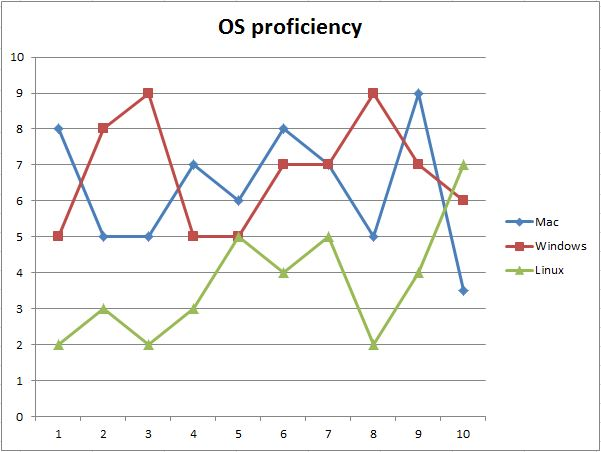
\includegraphics[width=0.75\textwidth]{./Images/Proficiency}
  \caption{Proficiency Values}
 \label{Proficiency}
\end{figure}

\begin{figure}[h!]
  \centering
    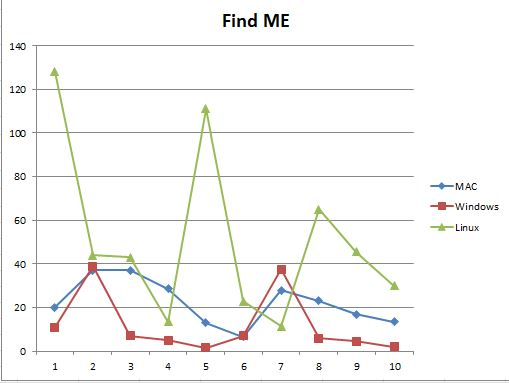
\includegraphics[width=0.75\textwidth]{./Images/Find_ME}
  \caption{Find Me search times}
 \label{Find}
\end{figure}
% JD: Use of graphs is noted and appreciated---you should compare yours with how
%     the graphs in the distributed published papers were structured.

\subsection{Task 1: Finding a File}
For this task a file titled Find ME was hidden within multiple layers of folders. The graph showing the different times it took to find the file is shown in Figure~\ref{Find}. For this task it seemed unanimous that all the users used the spotlight to find the file. This seemed to be the most efficient method to find the file and no one seemed to bother trying to search for the file through the folders. The same was done with Windows and once again search was heavily used. However once it came to Linux this was lost. By this point the subjects were used to using the search method and were seemed very determined to make it work. They tried and failed to find the file and again instead of trying to search through the folders they continued to try and use search. This shows that users have had sufficient experience with task such as this and realize that search is an effective method. The fact that all of the operating systems provide this functionality shows it has been noted to be helpful and something that is very user friendly and worth implementing.

\subsection{Task 2: Setting up Wi-Fi}
This task had the test subjects connect to the student Wi-Fi. The times are shown in Figure~\ref{Wi-Fi} In all the different operating systems the times were significantly shorter than the rest. In every operating system a there was found a familiar symbol for Wi-Fi. This would mean that people connect Wi-Fi to that symbol. In other words the symbol or anything remotely similar is considered synonymous to Wi-Fi and will attract the users attention to set up the Wi-Fi.

\begin{figure}[h!]
  \centering
    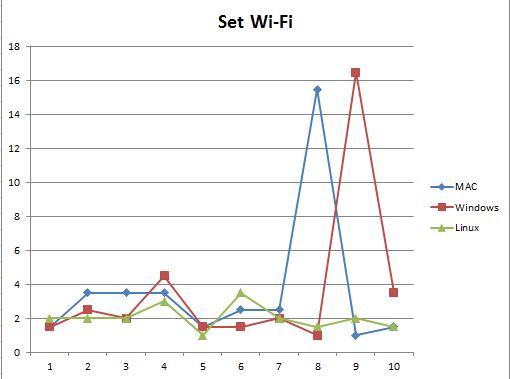
\includegraphics[width=0.75\textwidth]{./Images/Wi-Fi}
  \caption{Wi-Fi set-up times}
 \label{Wi-Fi}
\end{figure}


\subsection{Task 3: Calculator}
This task had very different results for every operating system. Figure~\ref{Calc} illustrates the time it took for this process. When it came to Mac some of the subjects knew about the simple gesture to get to the calculator widget. This is what caused fluctuations with the time of the Mac. Those who knew of the widget would get there in a couple of seconds whereas those who didn’t will take a while longer. As for windows everyone used the search method which immediately gave calculator when searched and allowed for a fast access to it. Linux however was the slowest. The user could not search for the calculator as they did with the other operating systems. This required the application tab to be chose first however it was somewhat hidden from view and so there was difficulty in getting to the calculator.

\begin{figure}[h!]
  \centering
    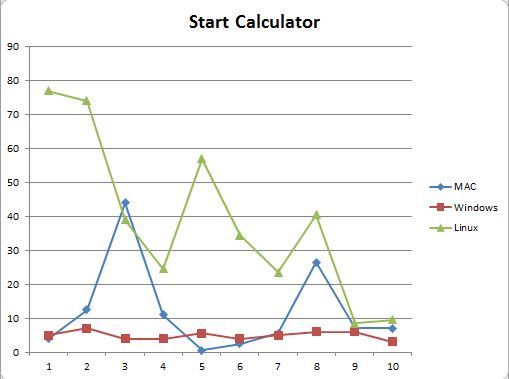
\includegraphics[width=0.75\textwidth]{./Images/Calculator}
  \caption{Calculator times}
 \label{Calc}
\end{figure}



\subsection{Data Summary}
Figure~\ref{Average} shows the average time values it took to complete each task in each operating system. One of the main trends that emerge is that Linux was the one that required the most time for every task except for Wi-Fi. None of the subjects were proficient in Linux except for one and so this experiment was probably their first experience with it. This meant that the experiment was actually a learning progress for them. Figure~\ref{Satis} shows the average satisfaction from a scale of 1 to 10 for the users with each Operating system. This chart shows that most people disliked Linux and felt it was bad with one subject even asking ``why would you ever use this.'' Figure~\ref{Satis} also shows that subjects were satisfied with the Mac operating system and its way of operating.

\begin{figure}[h!]
  \centering
    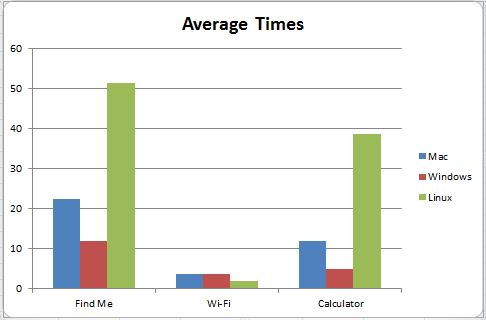
\includegraphics[width=0.75\textwidth]{./Images/Average_Times}
  \caption{Average Time Values}
 \label{Average}
\end{figure}

\begin{figure}[h!]
  \centering
    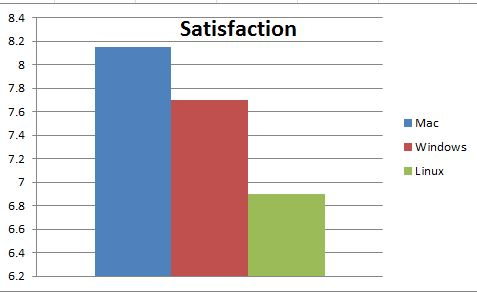
\includegraphics[width=0.75\textwidth]{./Images/Satisfaction}
  \caption{Average Satisfaction Values}
 \label{Satis}
\end{figure}

\section{Explanation of Results}


\subsection{Explaining: Finding a File}
All of the times for this task were relatively short. Most people have had some experience with finding a file. More than likely they use the search function as they know it will be easier to have their computer find the file for them than search for it themselves. Figure~\ref{SearchWin} shows the search for a Windows operating system. This can be easily found when the start button is pressed. This is a function that can be seen by the user every time they need to shut down their machine. They will be aware of its existence and because the location of the button is always in the same location users can easily find it and use it. Mac has a similar method except it can be used immediately as it can be found on the screen at all times. The problem that appeared with Linux is that users are accustomed to the search function searching through every file in the computer. Linux however has a dropdown menu to select specific locations to search for as can be seen in Figure ~\ref{SearchLinAfter}. Most users that were not accustomed with this and did not bother changing the location until attempting to search the same location 2-3 more times and failing to find the file.

% JD: Screencaps good. :)
\begin{figure}[h!]
  \centering
    
\includegraphics[width=0.75\textwidth]{./Images/Search_Windows}
  \caption{Windows Search Bar}
 \label{SearchWin}
\end{figure}

\begin{figure}[h!]
  \centering
    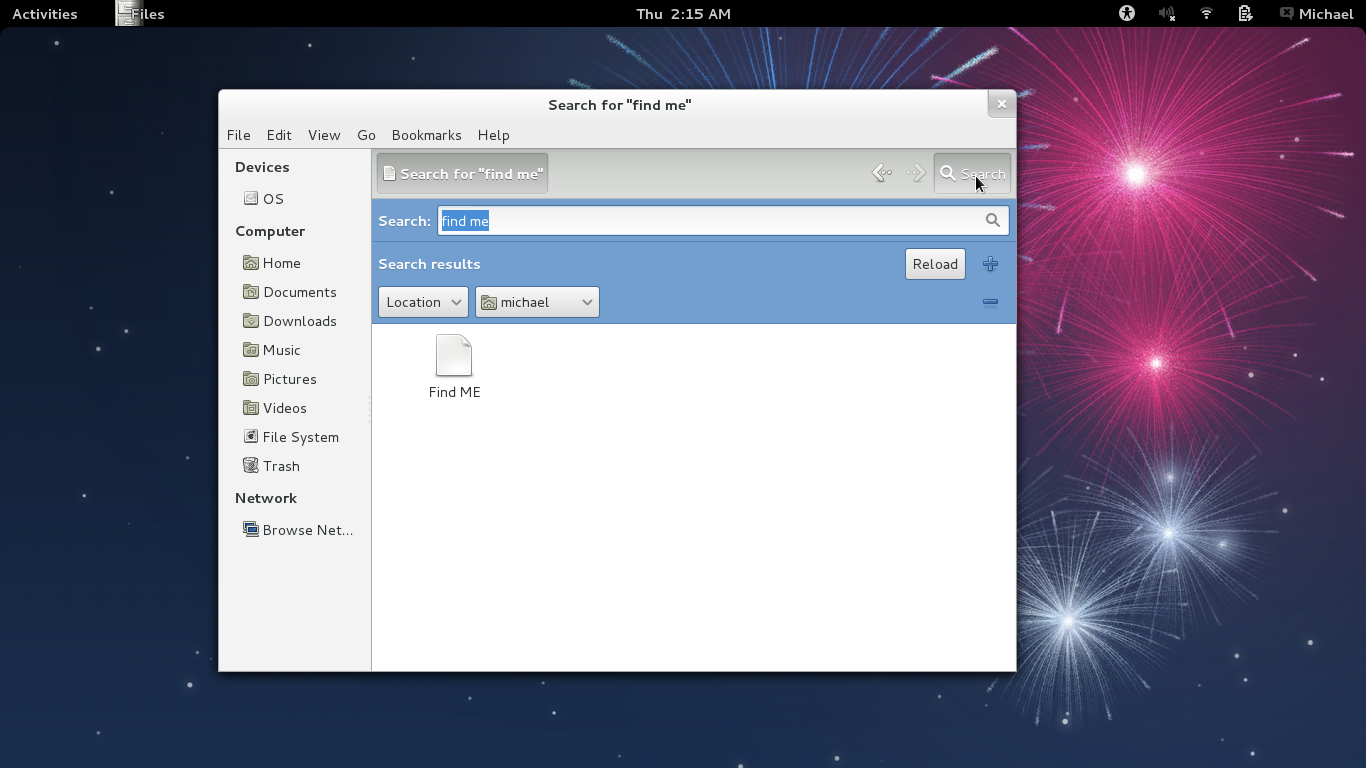
\includegraphics[width=0.75\textwidth]{./Images/Linux_Search_After}
  \caption{Linux after search has startedr}
 \label{SearchLinAfter}
\end{figure}

\subsection{Explaining: Setting up Wi-Fi}
Setting up Wi-Fi was the task that was completed in the least amount of time. The reason being that even though each system was different they all had some form of the Wi-Fi signal image as seen in Figure~\ref{WF}. This symbol or similar symbols have been universally accepted as the symbol Wi-Fi and thus the symbol to set the Wi-Fi. Figure~\ref{LinDesktop}shows a typical Linux desktop, the Wi-Fi symbol can be clearly seen in the top right corner of the desktop. This means the symbol can be easily seen and it is a symbol that portrays its purpose. This consistency across the systems demonstrates that it works and the results also show that it works in terms of being good interaction design. The user knows what to look for and a general area to look for.

\begin{figure}[h!]
  \centering
    
\includegraphics[width=0.5\textwidth]{./Images/Symbol_Wi-Fi}
  \caption{Wi-Fi symbol}
 \label{WF}
\end{figure}

\begin{figure}[h!]
  \centering
    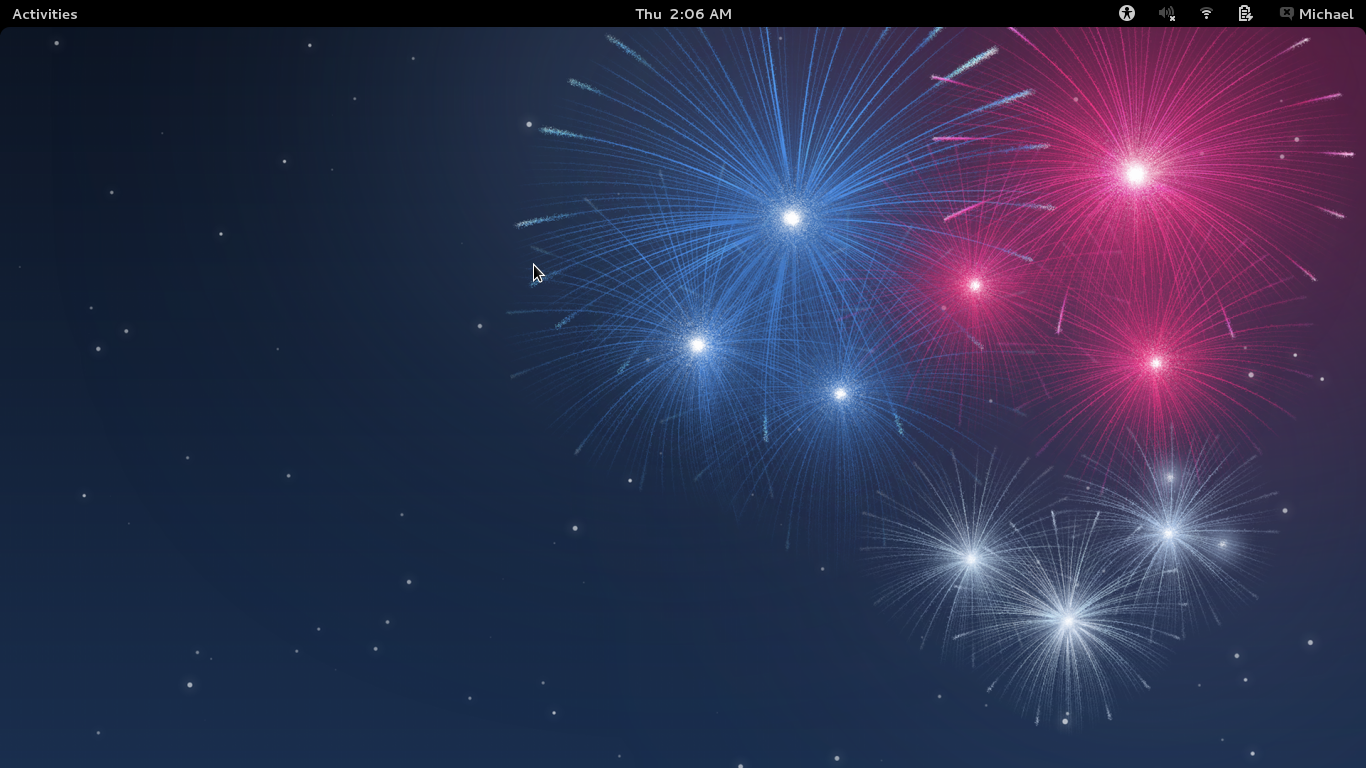
\includegraphics[width=0.75\textwidth]{./Images/Linux_Main}
  \caption{Linux Desktop}
 \label{LinDesktop}
\end{figure}

\subsection{Explaining: Getting to Calculator}
Calculator was different with each system, one could search, one had a quick gesture and the other required that a specific tab be pressed. Mac and Windows were easy to have the task accomplished. As was mentioned earlier the tabs are somewhat transparent and easy to miss. Most subjects had the chance to see the tabs while searching for the file. However it did not catch their attention causing them to overlook the applications tab which is where calculator would normally be found. The subject with the quickest Linux calculator time did so only because they happened to have spotted the application tab and knew where to search. Should this text be less transparent or even bigger it would be easier to spot and easier to target as stated by Fitt’s law.
% JD: Huh?  After the nice illustrations for the other tasks, the sudden dropoff
%     here is actually quite noticeable (with negative impact).  In particular,
%     I am not sure what is meant here by the "tabs" which were "easy to miss"---
%     a picture would have helped.

\section{Special Notes}
\subsection{Notes related to Experiment}
At some point during the experimentation it seems that the Find ME file was dragged to the desktop. Although it was placed on the desktop most subjects still went through the search method. This means they were simply not paying all that much attention to the desktop. There were two people however who did notice it and clicked it as soon as the timer began. That is what caused the two low times in finding the file for Windows. It should also be noted that the subject that stated they were proficient in Linux only had experience with Ubuntu and with Fedora being very different also had some difficulty with the Linux portion of the experiment.
% JD: That file-on-the-desktop oversight is actually a fairly major one, and strictly
%     speaking one should throw out the two non-search data points as invalid.  Lesson
%     learned presumably, and not to be repeated if you were to do this again? :)

\end{document}
